% CIFAR-10 Results Visualization
% Shows accuracy vs configuration

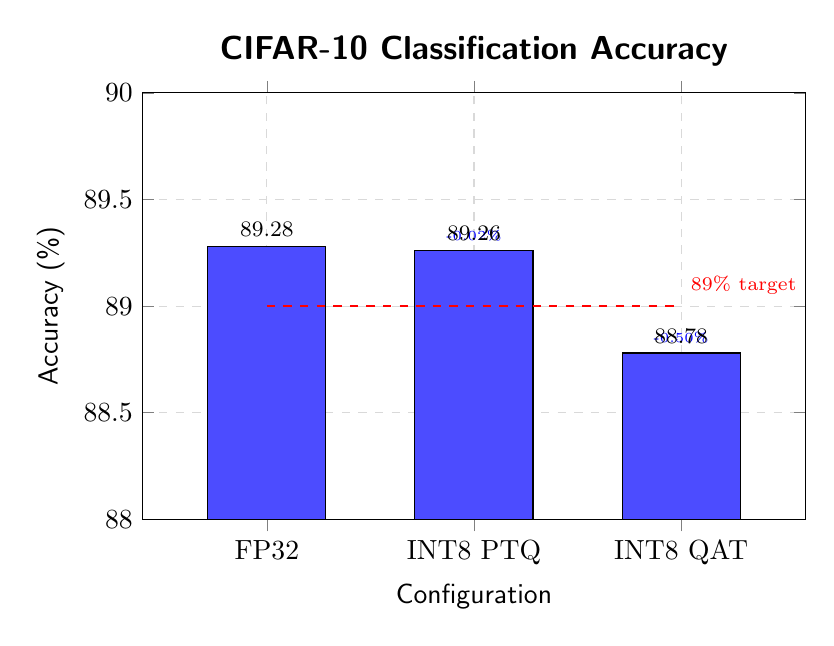
\begin{tikzpicture}
\begin{axis}[
    ybar,
    width=10cm,
    height=7cm,
    ylabel={Accuracy (\%)},
    xlabel={Configuration},
    symbolic x coords={FP32, INT8 PTQ, INT8 QAT},
    xtick=data,
    ymin=88,
    ymax=90,
    bar width=1.5cm,
    nodes near coords,
    nodes near coords align={vertical},
    every node near coord/.append style={font=\footnotesize},
    ylabel style={font=\sffamily},
    xlabel style={font=\sffamily},
    title={CIFAR-10 Classification Accuracy},
    title style={font=\large\sffamily\bfseries},
    enlarge x limits=0.3,
    legend style={at={(0.5,0.97)}, anchor=north},
    grid=major,
    grid style={dashed, gray!30},
]

\addplot[fill=blue!70, draw=black] coordinates {
    (FP32, 89.28)
    (INT8 PTQ, 89.26)
    (INT8 QAT, 88.78)
};

% Add target line at 89%
\draw[red, thick, dashed] (axis cs:FP32,89) -- (axis cs:INT8 QAT,89);
\node[font=\scriptsize, text=red, anchor=west] at (axis cs:INT8 QAT, 89.1) {89\% target};

% Annotate accuracy degradation
\node[font=\tiny, text=blue, anchor=south] at (axis cs:INT8 PTQ, 89.26) {-0.02\%};
\node[font=\tiny, text=blue, anchor=south] at (axis cs:INT8 QAT, 88.78) {-0.50\%};

\end{axis}
\end{tikzpicture}
